\documentclass{article}

\usepackage{graphicx}
\usepackage{rotating}
\usepackage{amsmath}
\usepackage{amssymb}
\usepackage{mathrsfs}
\usepackage{fancyhdr}
\usepackage{listings}
\usepackage{xcolor}
\usepackage{color}
\usepackage{amsfonts}
\usepackage{textcomp}
\usepackage{float}
\usepackage{neuralnetwork}
\usepackage{pgfplots}
\usepackage[sorting=none]{biblatex}
\usepackage[margin=1in]{geometry}
\usepackage[font={small,it}]{caption}
\usepackage{placeins}
\usepackage{tikz}
\usepackage{xepersian}

%\usepackage[left=2cm,right=2cm,top=2cm,bottom=2cm]{geometry}


\usetikzlibrary{decorations.pathreplacing}
\usetikzlibrary{fadings}

\pgfplotsset{width=8cm,compat=1.17}

%\DeclareMathOperator*{\btie}{\bowtie}
\addbibresource{bibliography.bib}
\settextfont[Scale=1.2]{B-NAZANIN.TTF}
\setlatintextfont[Scale=1]{Times New Roman}
\renewcommand{\baselinestretch}{1.5}
\pagestyle{fancy}
\fancyhf{}
\rhead{تکلیف سوم درس یادگیری عمیق}
\lhead{\thepage}
\rfoot{علیرضا ابره فروش}
\lfoot{9816603}
\renewcommand{\headrulewidth}{1pt}
\renewcommand{\footrulewidth}{1pt}
\newcommand{\Lagr}{\mathcal{L}}
\newcommand{\Mod}[1]{\ (\mathrm{mod}\ #1)}
%%%%%%%%%%
\lstset
{
    language=[latex]tex,
    basicstyle=\ttfamily,
    commentstyle=\color{black},
    columns=fullflexible,
    keepspaces=true,
    upquote=true,
    showstringspaces=false,
    morestring=[s]\\\%,
    stringstyle=\color{black},
}
%%%%%%%%%%
%beginMatlab
\definecolor{mygreen}{RGB}{28,172,0} % color values Red, Green, Blue
\definecolor{mylilas}{RGB}{170,55,241}
%endMatlab
\begin{document}
%beginMatlab
\lstset{language=Matlab,%
    %basicstyle=\color{red},
    breaklines=true,%
    morekeywords={matlab2tikz},
    keywordstyle=\color{blue},%
    morekeywords=[2]{1}, keywordstyle=[2]{\color{black}},
    identifierstyle=\color{black},%
    stringstyle=\color{mylilas},
    commentstyle=\color{mygreen},%
    showstringspaces=false,%without this there will be a symbol in the places where there is a space
    numbers=left,%
    numberstyle={\tiny \color{black}},% size of the numbers
    numbersep=9pt, % this defines how far the numbers are from the text
    emph=[1]{for,end,break},emphstyle=[1]\color{red}, %some words to emphasise
    %emph=[2]{word1,word2}, emphstyle=[2]{style},    
}
%endMatlab
\begin{titlepage}
\begin{center}

\includegraphics[width=0.4\textwidth]{figures/IUT Logo.png}\\
        
\LARGE
\textbf{دانشگاه صنعتی اصفهان}\\
\textbf{دانشکده مهندسی برق و کامپیوتر}\\
        
\vfill
        
\huge
\textbf{عنوان: تکلیف چهارم درس ریزپردازنده}\\
        
\vfill
        
\LARGE
\textbf{نام و نام خانوادگی: علیرضا ابره فروش}\\
\textbf{شماره دانشجویی: 9816603}\\
\textbf{نیم\,سال تحصیلی: پاییز 1400}\\
\textbf{مدرّس: دکتر عارف کریمی افشار}\\
\end{center}
\end{titlepage}


%\tableofcontents
\newpage


%1
\section{}
استفاده از تصاویر در شبکه‌های عصبی معمولی (\lr{MLP}) دارای مشکلاتی بود که با ظهور شبکه‌های عصبی کانولوشنی (\lr{CNN}) حل شد:
\begin{enumerate}

\item تعداد پارامترها و اتصالات:

در \lr{MLP}، هر نورون لایه ورودی با تمام نورون‌های لایه خروجی متصل بود. این اتصالات کامل منجر به افزایش سریع تعداد پارامترها می‌شد، که با تعداد بزرگ تصاویر (از نظر تعداد پیکسل) به سرعت غیرقابل مدیریت می‌شد.
    در \lr{CNN}، از لایه‌های کانولوشنی برای به اشتراک‌گذاری ویژگی‌ها در تصاویر استفاده می‌شود. این لایه‌ها با اعمال فیلترها (کرنل‌ها) به تصویر، ویژگی‌های مختلف را استخراج می‌کنند و این باعث کاهش تعداد پارامترها و اتصالات شبکه می‌شود. به عبارت دیگر، \lr{CNN} با استفاده از به اشتراک‌گذاری ویژگی‌ها، تعداد پارامترها را به شدت کاهش می‌دهد.

\item مقاومت به تغییرات مکانی:

\lr{MLP} به طور کامل حساس به تغییرات مکانی در تصویر بود. به عبارت دیگر، اگر یک الگو یا ویژگی در یک مکان خاص در تصویر وجود داشت، \lr{MLP} قادر به تشخیص آن در سایر نقاط تصویر نبود. \lr{CNN} با استفاده از لایه‌های کانولوشنی و استفاده از فیلترها، از این قابلیت برای شناسایی ویژگی‌ها در تمام تصویر به خوبی استفاده می‌کند. به این ترتیب، شبکه \lr{CNN} مقاوم‌تر به تغییرات مکانی در تصاویر می‌شود و توانایی خود را در تشخیص الگوها و ویژگی‌ها در مکان‌های مختلف تصویر افزایش می‌دهد.

\item عدم حفظ ساختار مکانی:
\lr{MLP}، ساختار مکانی تصویر حذف می‌شد و هر پیکسل به عنوان یک ویژگی مستقل در نظر گرفته می‌شد. این عدم حفظ ساختار مکانی اطلاعات مهمی را از دست می‌داد، به خصوص برای تصاویری که الگوها و اطلاعات مکانی مهمی دارند.
    \lr{CNN} با استفاده از لایه‌های کانولوشنی و اعمال فیلترها، قابلیت حفظ ساختار مکانی را به شبکه اضافه کرده و اجازه می‌دهد تا ویژگی‌ها به صورت محلی در تصویر استخراج شوند. این امکان باعث می‌شود که شبکه بتواند اطلاعات مکانی را مورد توجه قرار داده و الگوهای مکانی پیچیده‌تری را در تصاویر تشخیص دهد.

\item تفسیرپذیری پایین:

    \lr{MLP}‌ها به دلیل تعداد بسیار زیاد پارامترها، به صورت کلی دارای تفسیرپذیری پایین بودند. یعنی مشخص کردن دقیق اینکه شبکه چگونه تصمیمات خود را اتخاذ کرده است، معمولاً مشکل بود.
    \lr{CNN} با تعداد کمتر پارامترها و استفاده از فیلترها، قابلیت تفسیرپذیری بیشتری دارد. این به این معناست که می‌توان بهتر فهمید که شبکه در تصمیم‌گیری‌های خود چگونه از ویژگی‌ها استفاده می‌کند.

\item حساسیت به اندازه تصویر:

    \lr{MLP}‌ها به صورت ثابت و بدون توجه به ابعاد تصویر (مثلاً ابعاد ورودی ثابت دارای تعداد ثابت نورون‌ها) عمل می‌کردند. این باعث می‌شد که اگر تصویر ورودی ابعاد متفاوتی داشته باشد، شبکه به طور مستقیم با آن کار نکند.
    \lr{CNN} با استفاده از لایه‌های کانولوشنی می‌تواند به تصاویر با ابعاد مختلف و با استفاده از فیلترهای متفاوت به خوبی پاسخ دهد و حساسیت کمتری نسبت به ابعاد تصویر نشان دهد.

\item برخورد با تعداد زیاد پارامترها:

    با افزایش اندازه تصاویر، تعداد پارامترهای مورد نیاز برای یک \lr{MLP} به صورت نمایی افزایش می‌یابد. این موضوع باعث ایجاد مدل‌های بسیار پیچیده و سنگین می‌شود که دشواری در آموزش، نگهداری و استفاده از آن‌ها را افزایش می‌دهد.

\item عدم توانایی در مدل‌سازی ویژگی‌های سلسله‌مراتبی:

    \lr{MLP} به طور مستقیم قادر به مدل‌سازی ویژگی‌های سلسله‌مراتبی و پیچیده تصاویر نیستند. به عبارت دیگر، آن‌ها قادر به استخراج ویژگی‌های موقعیت مکانی، الگوها و ساختارهای سلسله‌مراتبی نیستند که در بینایی ماشین بسیار مهم است.

\item حساسیت به تغییرات شدت نور و ظروف نوری:

    \lr{MLP} در مقابل تغییرات شدت نور و ظروف نوری حساس هستند. این به این معناست که تصاویر با نور متفاوت یا ظروف نوری متفاوت ممکن است تأثیر زیادی بر عملکرد \lr{MLP} داشته باشند.

\item اشتباه‌زاهای غیرقابل کنترل:

    به دلیل تعداد بالای پارامترها و عدم استفاده از الگوهای مکانی، \lr{MLP}‌ها ممکن است به آموزش بیش از حد به داده‌ها وابسته شوند و اشتباه‌زاهای غیرقابل کنترل در عملکرد آن‌ها ایجاد شود.

\item کارایی ضعیف در مسائل تشخیص الگو:

    در مسائل تشخیص الگو و ویژگی‌های پیچیده در تصاویر، \lr{MLP}‌ها عملکرد ضعیفی دارند. زیرا این مدل‌ها نمی‌توانند ویژگی‌های سلسله‌مراتبی و پیچیده را به صورت کامل مدل کنند.

شبکه‌های عصبی کانولوشنی (\lr{CNN}) با توجه به مزایایی که در پردازش تصاویر دارند، این مشکلات را به حداقل می‌رسانند و بهبودهای مهمی را در زمینه بینایی ماشین و پردازش تصویر به ارمغان آورده‌اند.
\end{enumerate}

%2
\section{}

%3
\section{}

%4
\section{}
\begin{latin}
\begin{figure}[H]
	\centering
	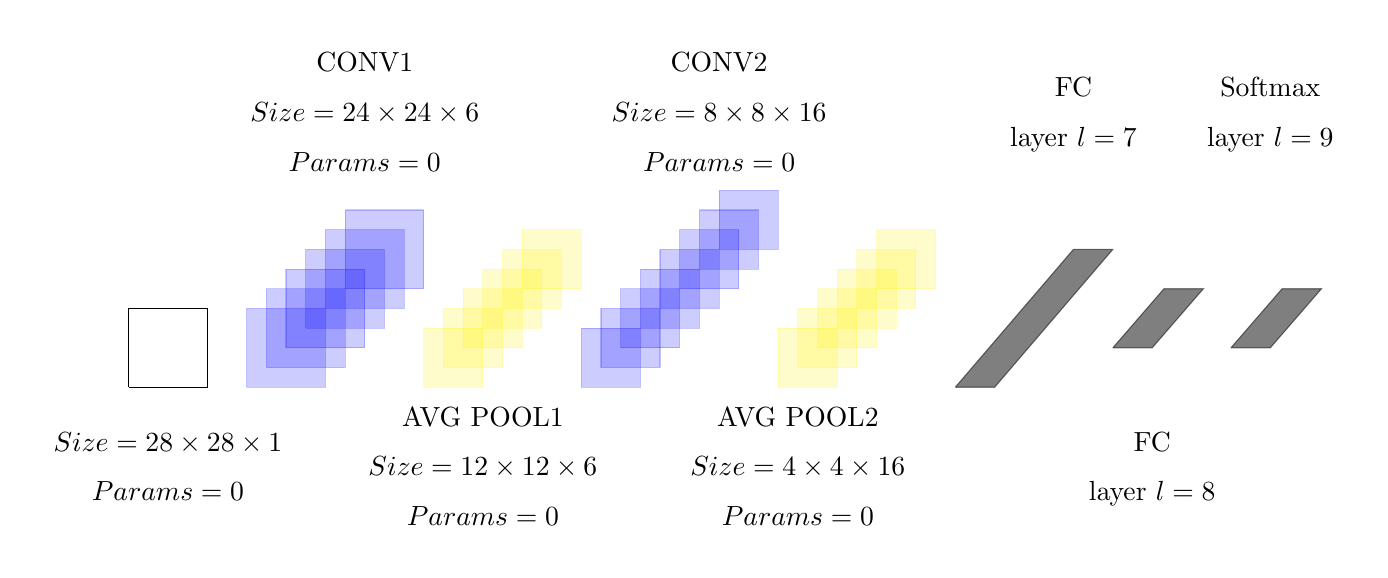
\begin{tikzpicture}
		\node at (0.5,-1){\begin{tabular}{c}$Size = 28 \times 28 \times 1$\\$Params = 0$\end{tabular}};
		
		\draw (0,0) -- (1,0) -- (1,1) -- (0,1) -- (0,0);
		
		\node at (3,3.5){\begin{tabular}{c}CONV1\\$Size = 24 \times 24 \times 6$\\$Params = 0$\end{tabular}};
		
		\draw[fill=blue,opacity=0.2,draw=blue] (2.75,1.25) -- (3.75,1.25) -- (3.75,2.25) -- (2.75,2.25) -- (2.75,1.25);
		\draw[fill=blue,opacity=0.2,draw=blue] (2.5,1) -- (3.5,1) -- (3.5,2) -- (2.5,2) -- (2.5,1);
		\draw[fill=blue,opacity=0.2,draw=blue] (2.25,0.75) -- (3.25,0.75) -- (3.25,1.75) -- (2.25,1.75) -- (2.25,0.75);
		\draw[fill=blue,opacity=0.2,draw=blue] (2,0.5) -- (3,0.5) -- (3,1.5) -- (2,1.5) -- (2,0.5);
		\draw[fill=blue,opacity=0.2,draw=blue] (1.75,0.25) -- (2.75,0.25) -- (2.75,1.25) -- (1.75,1.25) -- (1.75,0.25);
		\draw[fill=blue,opacity=0.2,draw=blue] (1.5,0) -- (2.5,0) -- (2.5,1) -- (1.5,1) -- (1.5,0);
		
		\node at (4.5,-1){\begin{tabular}{c}AVG POOL1\\$Size = 12 \times 12 \times 6$\\$Params = 0$\end{tabular}};
		
		\draw[fill=yellow,opacity=0.2,draw=yellow] (5,1.25) -- (5.75,1.25) -- (5.75,2) -- (5,2) -- (5,1.25);
		\draw[fill=yellow,opacity=0.2,draw=yellow] (4.75,1) -- (5.5,1) -- (5.5,1.75) -- (4.75,1.75) -- (4.75,1);
		\draw[fill=yellow,opacity=0.2,draw=yellow] (4.5,0.75) -- (5.25,0.75) -- (5.25,1.5) -- (4.5,1.5) -- (4.5,0.75);
		\draw[fill=yellow,opacity=0.2,draw=yellow] (4.25,0.5) -- (5,0.5) -- (5,1.25) -- (4.25,1.25) -- (4.25,0.5);
		\draw[fill=yellow,opacity=0.2,draw=yellow] (4,0.25) -- (4.75,0.25) -- (4.75,1) -- (4,1) -- (4,0.25);
		\draw[fill=yellow,opacity=0.2,draw=yellow] (3.75,0) -- (4.5,0) -- (4.5,0.75) -- (3.75,0.75) -- (3.75,0);
		
		\node at (7.5,3.5){\begin{tabular}{c}CONV2\\$Size = 8 \times 8 \times 16$\\$Params = 0$\end{tabular}};
		
		\draw[fill=blue,opacity=0.2,draw=blue] (7.5,1.75) -- (8.25,1.75) -- (8.25,2.5) -- (7.5,2.5) -- (7.5,1.75);
		\draw[fill=blue,opacity=0.2,draw=blue] (7.25,1.5) -- (8,1.5) -- (8,2.25) -- (7.25,2.25) -- (7.25,1.5);
		\draw[fill=blue,opacity=0.2,draw=blue] (7,1.25) -- (7.75,1.25) -- (7.75,2) -- (7,2) -- (7,1.25);
		\draw[fill=blue,opacity=0.2,draw=blue] (6.75,1) -- (7.5,1) -- (7.5,1.75) -- (6.75,1.75) -- (6.75,1);
		\draw[fill=blue,opacity=0.2,draw=blue] (6.5,0.75) -- (7.25,0.75) -- (7.25,1.5) -- (6.5,1.5) -- (6.5,0.75);
		\draw[fill=blue,opacity=0.2,draw=blue] (6.25,0.5) -- (7,0.5) -- (7,1.25) -- (6.25,1.25) -- (6.25,0.5);
		\draw[fill=blue,opacity=0.2,draw=blue] (6,0.25) -- (6.75,0.25) -- (6.75,1) -- (6,1) -- (6,0.25);
		\draw[fill=blue,opacity=0.2,draw=blue] (5.75,0) -- (6.5,0) -- (6.5,0.75) -- (5.75,0.75) -- (5.75,0);
		
		\node at (8.5,-1){\begin{tabular}{c}AVG POOL2\\$Size = 4 \times 4 \times 16$\\$Params = 0$\end{tabular}};
		
		\draw[fill=yellow,opacity=0.2,draw=yellow] (9.5,1.25) -- (10.25,1.25) -- (10.25,2) -- (9.5,2) -- (9.5,1.25);
		\draw[fill=yellow,opacity=0.2,draw=yellow] (9.25,1) -- (10,1) -- (10,1.75) -- (9.25,1.75) -- (9.25,1);
		\draw[fill=yellow,opacity=0.2,draw=yellow] (9,0.75) -- (9.75,0.75) -- (9.75,1.5) -- (9,1.5) -- (9,0.75);
		\draw[fill=yellow,opacity=0.2,draw=yellow] (8.75,0.5) -- (9.5,0.5) -- (9.5,1.25) -- (8.75,1.25) -- (8.75,0.5);
		\draw[fill=yellow,opacity=0.2,draw=yellow] (8.5,0.25) -- (9.25,0.25) -- (9.25,1) -- (8.5,1) -- (8.5,0.25);
		\draw[fill=yellow,opacity=0.2,draw=yellow] (8.25,0) -- (9,0) -- (9,0.75) -- (8.25,0.75) -- (8.25,0);
		
		\node at (12,3.5){\begin{tabular}{c}FC\\layer $l = 7$\end{tabular}};
		
		\draw[fill=black,draw=black,opacity=0.5] (10.5,0) -- (11,0) -- (12.5,1.75) -- (12,1.75) -- (10.5,0);
		
		\node at (13,-1){\begin{tabular}{c}FC\\layer $l = 8$\end{tabular}};
		
		\draw[fill=black,draw=black,opacity=0.5] (12.5,0.5) -- (13,0.5) -- (13.65,1.25) -- (13.15,1.25) -- (12.5,0.5);

		\node at (14.5,3.5){\begin{tabular}{c}Softmax\\layer $l = 9$\end{tabular}};
		
		\draw[fill=black,draw=black,opacity=0.5] (14,0.5) -- (14.5,0.5) -- (15.15,1.25) -- (14.65,1.25) -- (14,0.5);
	\end{tikzpicture}
	\caption{}
	\label{fig:traditional-convolutional-network}
\end{figure}

$
\text{size after applying convolution layer} = \left\lfloor \frac{n + 2p - f}{s} + 1 \right\rfloor \times \left\lfloor \frac{n + 2p - f}{s} + 1 \right\rfloor \times k
$

\subsection*{Input Layer:}
\begin{itemize}
    \item Size: $28 \times 28 \times 1$
    \item Params: $0$
    \item Number of Channels: 1
\end{itemize}

\subsection*{CONV1 Layer:}
\begin{itemize}
    \item Filter size: $5 \times 5$
    \item Stride: 1
    \item Number of filters ($k$): 6
    \item Padding: 0
    \item Size: $\left\lfloor \frac{28 + 2 \times 0 - 5}{1} + 1 \right\rfloor \times \left\lfloor \frac{28 + 2 \times 0 - 5}{1} + 1 \right\rfloor \times 6 = 24 \times 24 \times 6$
    \item Params: $(5 \times 5 \times 1 + 1) \times 6 = 156$ (weights + bias for each filter)
\end{itemize}

\subsection*{Average Pooling Layer 1:}
\begin{itemize}
    \item Filter size: $2 \times 2$
    \item Stride: 2
    \item Size: $\left\lfloor \frac{24 + 2 \times 0 - 2}{2} + 1 \right\rfloor \times \left\lfloor \frac{24 + 2 \times 0 - 2}{2} + 1 \right\rfloor \times 6 = 12 \times 12 \times 6$
    \item Params: $0$
\end{itemize}

\subsection*{CONV2 Layer:}
\begin{itemize}
    \item Filter size: $5 \times 5$
    \item Stride: 1
    \item Number of filters ($k$): 16
    \item Padding: 0
    \item Size: $\left\lfloor \frac{12 + 2 \times 0 - 5}{1} + 1 \right\rfloor \times \left\lfloor \frac{12 + 2 \times 0 - 5}{1} + 1 \right\rfloor \times 16 = 8 \times 8 \times 16$
    \item Params: $(5 \times 5 \times 6 + 1) \times 16 = 2416$ (weights + bias for each filter)
\end{itemize}

\subsection*{Average Pooling Layer 2:}
\begin{itemize}
    \item Filter size: $2 \times 2$
    \item Stride: 2
    \item Size: $\left\lfloor \frac{8 + 2 \times 0 - 2}{2} + 1 \right\rfloor \times \left\lfloor \frac{8 + 2 \times 0 - 2}{2} + 1 \right\rfloor \times 16 = 4 \times 4 \times 16$
    \item Params: $0$
\end{itemize}

\subsection*{FC1 Layer (Fully Connected):}
\begin{itemize}
    \item Number of neurons: 128
    \item Params: $(4 \times 4 \times 16 + 1) \times 128 = 32896$ (weights + bias for each neuron)
\end{itemize}

\subsection*{FC2 Layer (Fully Connected):}
\begin{itemize}
    \item Number of neurons: 64
    \item Params: $(128 + 1) \times 64 = 8256$ (weights + bias for each neuron)
\end{itemize}

\subsection*{Softmax Layer:}
\begin{itemize}
    \item Number of neurons: 10 (assuming classification)
    \item Params: $(64 + 1) \times 10 = 650$ (weights + bias for each class)
\end{itemize}

$\textbf{Sum Parameters} = 156 + 2416 + 32896 + 8256 + 650 = 44374$

\end{latin}


%5
\section{}

%6
\section{}

%7
\section{}

%%%%%%%%%%%%%%%%%%%%%%%%%%%%%%%%%%%
%%%%%%%%%%%%%%%%%%%%%%%%%%%%%%%%%%%
%%%%%%%%%%%%%%%%%%%%%%%%%%%%%%%%%%%



\section*{منابع}
\renewcommand{\section}[2]{}%
\begin{thebibliography}{99} % assumes less than 100 references
%چنانچه مرجع فارسی نیز داشته باشید باید دستور فوق را فعال کنید و مراجع فارسی خود را بعد از این دستور وارد کنید


\begin{LTRitems}

\resetlatinfont

\bibitem{b1} https://www.shiksha.com/online-courses/articles/relu-and-sigmoid-activation-function/
\bibitem{b1} https://medium.com/@amanatulla1606/vanishing-gradient-problem-in-deep-learning-understanding-intuition-and-solutions-da90ef4ecb54
\bibitem{b1} https://en.wikipedia.org/wiki/Rectifier\_(neural\_networks)
\bibitem{b1} https://wandb.ai/ayush-thakur/dl-question-bank/reports/ReLU-vs-Sigmoid-Function-in-Deep-Neural-Networks--VmlldzoyMDk0MzI
\bibitem{b1} https://medium.com/swlh/why-are-neural-nets-non-linear-a46756c2d67f
\end{LTRitems}

\end{thebibliography}


\end{document}
